\documentclass[12pt,a4paper]{article}
 
                               
\usepackage[T1]{fontenc} % So we can use pretty T1 fonts
\usepackage{libertine}
 
\usepackage[margin=0.5in]{geometry}
\usepackage{amsmath,amssymb,amsfonts}
\usepackage{graphicx}
\usepackage{textcomp}
\usepackage{soul}
\usepackage{hyperref}
\usepackage{xcolor}
\usepackage{caption}
\usepackage{booktabs}
\usepackage{algorithm}
\usepackage{algorithmic}
%\usepackage{helvet}
%\usepackage{courier}
\usepackage{mathtools}
\usepackage{pifont}
\usepackage{dashbox}
\usepackage{xspace}
\usepackage{color}
\usepackage{multirow}
\usepackage{url}
%\usepackage{extsizes}
% the following package is optional:
\usepackage{latexsym}
%\usepackage{mathptmx}
\usepackage{stmaryrd}
\usepackage{enumitem}
\newtheorem{definition}{Definition}
\setlength\parindent{0pt}


\newcommand{\alc}{$\mathcal{ALC}$\xspace}
\newcommand{\el}{$\mathcal{EL}$\xspace}
%para nao ficar o retangulo em volta dos links, apenas muda a cor dos caracteres
\hypersetup{ colorlinks,
linkcolor=blue,
filecolor=blue,
urlcolor=blue,
citecolor=blue }

% altera a fonte nas legendas das figuras
%\usepackage[font=small,format=plain,labelfont=bf,up,textfont=times]{caption}
 

\newenvironment{problem}[2][{\color{red}Question}]{\begin{trivlist}
\item[\hskip \labelsep {\bfseries #1}\hskip \labelsep {\bfseries #2.}]}{\end{trivlist}}

\newenvironment{solution}[2][{\color{blue}Model Solution}]{\begin{trivlist}
\item[\hskip\labelsep {\bfseries #1}\hskip \labelsep {\bfseries #2.}]}{\end{trivlist}}

\setlength{\parskip}{0,3em}  %altera o espaco entre dois paragrafos
\renewcommand{\baselinestretch}{1.1} %altera o espacamento entre as linhas
 
\begin{document}


\title{{\color{blue}KRP --- Assignment 1}}
\author{Instructor: Yizheng Zhao}

 
\maketitle

\textbf{$\star$~\textcolor{gray}{This assignment, due on \underline{\textcolor{blue}{31st March at 23:59}}, contributes to 10\% of the total mark of the course.}}



\begin{problem}{{\color{red}1}}
\textbf{Manchester Syntax}\\
(1) Given the following ontology definition:
\begin{itemize}
\item[] Class: LivestockOwner
\item[] \quad SubClassOf: Person that hasLivestock some Cow and hasLivestock only (Cow or Sheep)
\item[] Class: Cow
\item[] \quad SubClassOf: Animal
\item[] Class: Dog
\item[] \quad SubClassOf: Animal
\item[] Individual: Tom
\item[] \quad Types: LivestockOwner
\item[] \quad Facts: hasLivestock Timo
\item[] Individual: Timo
\item[] \quad Types: not Sheep
\item What additional information do we know about Timo?
\end{itemize}


(2) Given the following ontology definition:
\begin{itemize}
\item[] Class: LivestockOwner
\item[] \quad SubClassOf: Person that hasLivestock some Cow and hasLivestock some Sheep
\item[] Class: Cow
\item[] \quad SubClassOf: Animal
\item[] Class: Sheep
\item[] \quad SubClassOf: Animal
\item[] Individual: Tom
\item[] \quad Types: LivestockOwner
\item[] \quad Facts: hasLivestock Timo hasLivestock Fido
\item[] Individual: Timo
\item[] \quad Types: Cow
\item[] Individual: Fido
\item Is Fido a Dog?
\end{itemize}


(3) Given the following ontology definition:
\begin{itemize}
\item[] Class: LivestockOwner
\item[] \quad SubClassOf: Person that hasLivestock some Cow
\item Is owning a Cow enough to recognize a Person as a LivestockOwner?
\end{itemize}


(4) Given the following ontology definition:
\begin{itemize}
\item[] Class: LivestockOwner
\item[] \quad SubClassOf: Person that hasLivestock some Cat and hasLivestock only Cat
\item How many Cows does a LivestockOwner have as Livestocks?
\end{itemize}
\end{problem}



\begin{problem}{{\color{red}2}}
\textbf{ALC Extensions \& FOL}\\
Consider the following sentences:
\begin{enumerate}
    \item[(1)] ML is an AI course taught by ZZH, a professor working at NJU
    \item[(2)] NJU is a university whose members are a school or a department
    \item[(3)] NJU has at least 30,000 students
    \item[(4)] All members of AI School are undergraduates, graduates, or teachers
    \item[(5)] The domain of the relation ``citizenOf'' consists of countries
\end{enumerate}
\begin{itemize}
    \item Translate these sentences into one or multiple SHOIQ inclusions
    \item Translate the LAST TWO inclusions into equivalent first-order logic
\end{itemize}

\end{problem}

\begin{problem}{{\color{red}3}}
\textbf{DL Semantics}\\
Prove or disprove the following statements:
\begin{itemize}
    \item There is an ontology that has only finite models.
    \item Every ontology has either no model or infinite many models.
    \item A satisfiable class must always have a non-empty interpretation.
    \item An unsatisfiable class may have a non-empty interpretation in some models.
    \item An unsatisfiable class will be a subclass of any other class.
\end{itemize}
\end{problem}


\begin{problem}{{\color{red}4}}
\textbf{Interpretation as Graph}\\
Consider the following graph $G$:
{\begin{figure}[ht]
    \centering
    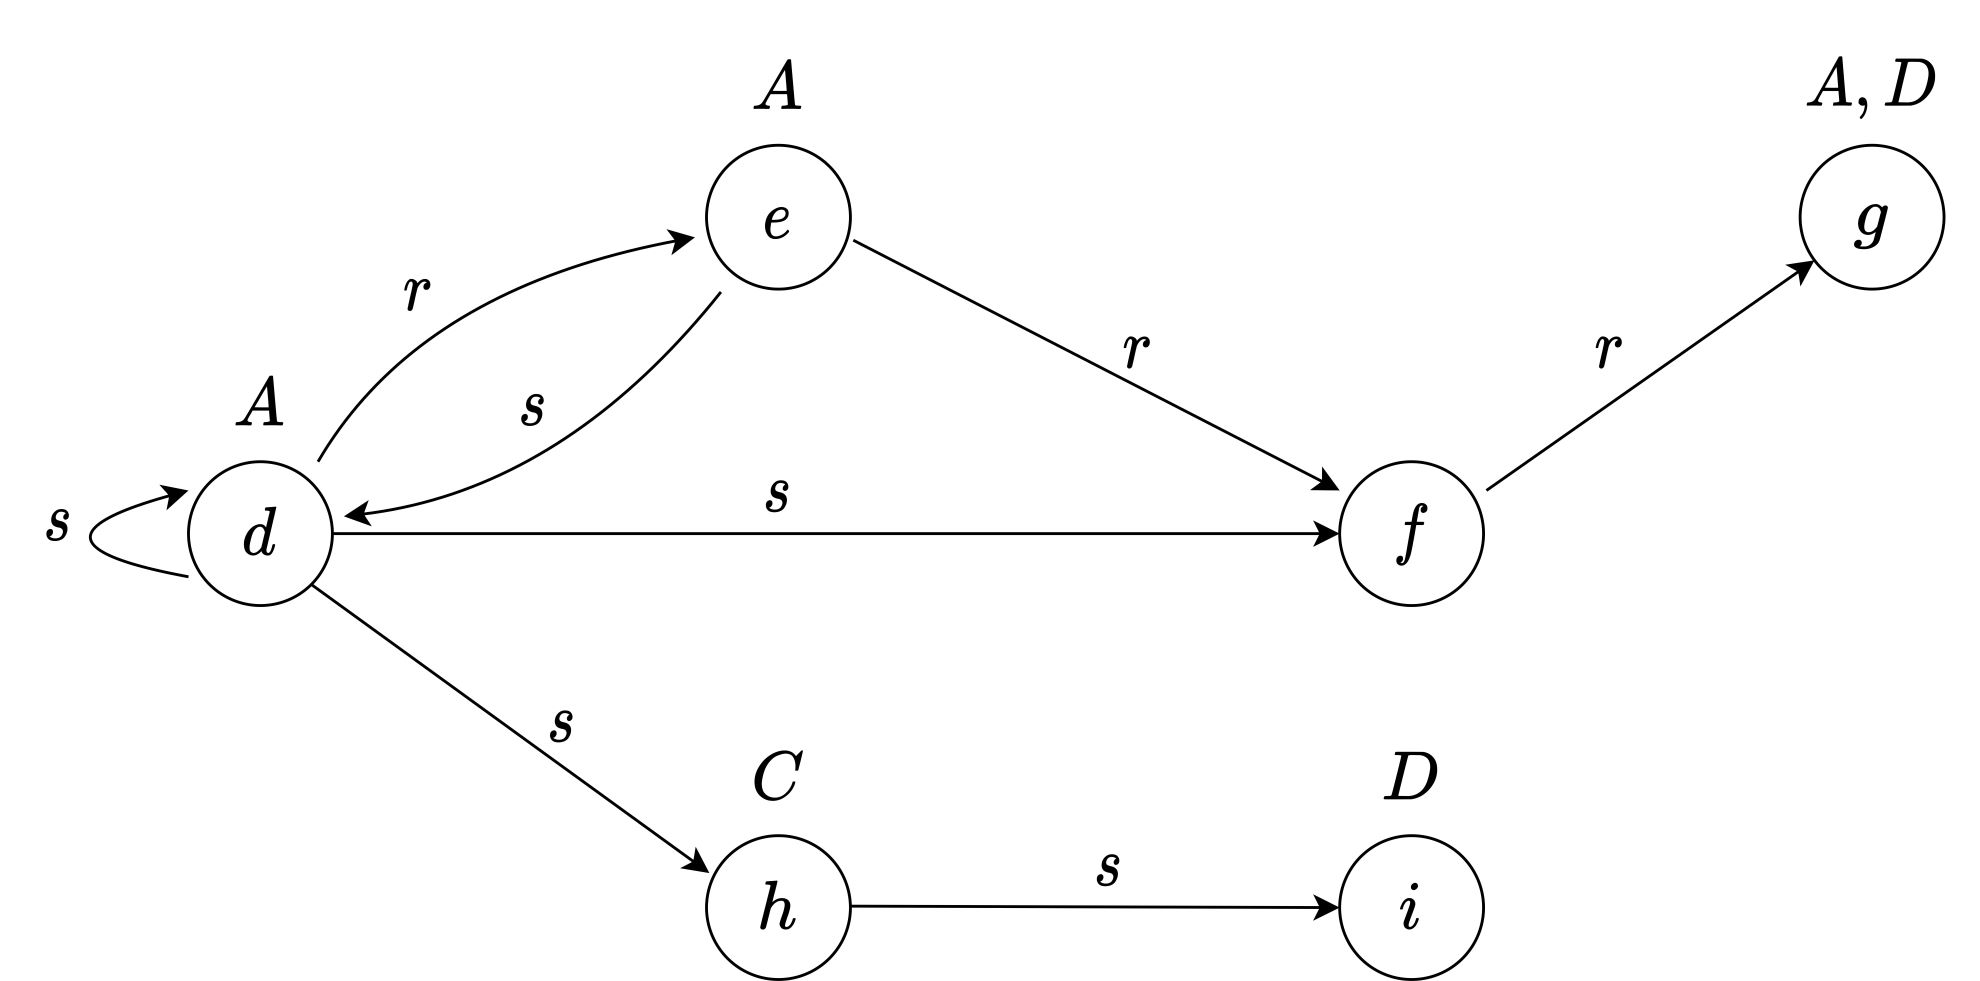
\includegraphics[width=0.55\columnwidth]{graph-min.jpg}
\end{figure}}
and the following set of concepts $S_{C}$:
\begin{enumerate}
    \item $\exists r.(A\sqcup B)$
    \item $\exists s.\exists s.\neg A$
    \item $\neg A\sqcap\neg B$
    \item $\forall r.(A\sqcup B)$
    \item $\leq{1}{s}.\top$
\end{enumerate}
First, we read the graph $G$ as an interpretation, where the vertices are elements of the domain and the labels of vertices and edges result from the interpretation function.
\begin{itemize}
    \item List for each of the concepts in $S_{C}$ which elements of the domain they have as instances.
\end{itemize}
\end{problem}


\begin{problem}{{\color{red}5}}
\textbf{DL Semantics}\\
(1) Consider the interpretation $\mathcal{I}$ defined by:
\begin{itemize}
    \item[] $\Delta^{\mathcal{I}}=\{a, b, c, d, e\}$
    \item[] $P^{\mathcal{I}}=\{a, b, d\}$
    \item[] $Q^{\mathcal{I}}=\{d, e\}$
    \item[] $r^{\mathcal{I}}=\{(a, b), (a, d), (d, e)\}$ 
\end{itemize}

Determine the following sets:
\begin{itemize}
    \item $(Q~\sqcap\geq{2}{r}.P)^{\mathcal{I}}$
    \item $(\forall r.Q)^{\mathcal{I}}$
    \item $(\neg\exists r.Q)^{\mathcal{I}}$
    \item $(\forall r.\top\sqcap\exists r^{-}.P)^{\mathcal{I}}$
    \item $(\exists r^{-}.\bot)^{\mathcal{I}}$
\end{itemize}

(2) Consider the interpretation $\mathcal{I}$ defined by:
\begin{itemize}
    \item[] $\Delta^{\mathcal{I}}=\{1,2,3,4,5,6\}$
    \item[] $A^{\mathcal{I}}=\{1,2\}$
    \item[] $B^{\mathcal{I}}=\{3,4,5,6\}$
    \item[] $r^{\mathcal{I}}=\{(1,3),(1,5),(2,6)\}$
\end{itemize}
Which of the following are true?
\begin{itemize}
    \item $\mathcal{I}\models A\equiv\exists r.B$
    \item $\mathcal{I}\models A\sqcap B\sqsubseteq\top$
    \item $\mathcal{I}\models \exists r.A\sqsubseteq A\sqcap B$
    \item $\mathcal{I}\models \top\sqsubseteq B$
    \item $\mathcal{I}\models B\sqsubseteq\exists r.A$
\end{itemize}
\end{problem}


\begin{problem}{{\color{red}6}}
\textbf{DL Semantics}\\
Which of the following statements hold:
\begin{itemize}
    \item if $C\sqsubseteq D$ holds, then $\exists r.C\sqsubseteq\exists r.D$ holds.
    \item $\exists r.C$ is equivalent to $\leq{1}{r}.\top$.
    \item $\leq{0}{r}.\top$ is equivalent to $\forall r.\bot$.
    \item $\forall r.(A\sqcup B)$ is equivalent to $(\forall r.A)\sqcup(\forall r.B)$.
    \item $\exists r.(A\sqcup B)$ is equivalent to $(\exists r.A)\sqcup(\exists r.B)$.
\end{itemize}
Justify your answers.
\end{problem}


\begin{problem}{{\color{red}7}}
\textbf{DL Semantics}\\
Let $\mathcal{T}=\{\textsf{Parent}\sqsubseteq\exists\textsf{hasChild}.\textsf{Person}, \textsf{Mother}\sqsubseteq\textsf{Parent}\}$.
\begin{itemize}
\item Show that $\mathcal{T}\not\models\textsf{Parent}\sqsubseteq\textsf{Mother}$ by giving an interpretation $\mathcal{I}$ such that $\mathcal{I}\models\mathcal{T}$ and $\mathcal{I}\not\models\textsf{Parent}\sqsubseteq\textsf{Mother}$.
\end{itemize}
\end{problem}


\begin{problem}{{\color{red}8}}
\textbf{DL Semantics}\\
Let $\mathcal{T}$ be an $\mathcal{ALC}$ TBox, which is a finite set of concept inclusions. Let $X$ and $Y$ be complex $\mathcal{ALC}$ concepts (note that a complex concept can also be an atomic concept). Show that:
\begin{itemize}
    \item $X\sqsubseteq_{\mathcal{T}}Y$ if and only if $X\sqcap\neg Y$ is not satisfiable with respect to $\mathcal{T}$.
    \item $X$ is satisfiable with respect to $\mathcal{T}$ if and only if $X\not\sqsubseteq\bot$.
\end{itemize}
\end{problem}


\begin{problem}{{\color{red}9}}
\textbf{Get to know Prot$\acute{e}$g$\acute{e}$}
Choose from the File menu ``Open from URL'' to load the pizza ontology into Prot$\acute{e}$g$\acute{e}$ \url{https://protege.stanford.edu/ontologies/pizza/pizza.owl}. Activate the view ``Ontology metric'', which is accessible from the menu ``Window'' $\rightarrow$ ``Views'' $\rightarrow$ ``Ontology view'' $\rightarrow$ ``Ontology metrics''.
\begin{itemize}
    \item What is the axiom count and what is the logical axiom count? Why does it differ? (To find out details of the pizza ontology, use the tabs for ``Entities'', ``Classes'', and ``'Object properties').
    \item Find axioms in the pizza ontology that respectively
    \begin{itemize}
        \item use nominals,
        \item use negations,
        \item declare a sub-property of an object property, and
        \item declare an inverse property.
    \end{itemize}
    \item Start the reasoner from the menu ``Reasoner''. In the tab ``Classes'' in the view for ``Class hierarchy'' the class ``Ice Cream'' is shown in red. Why?
    \item What are the inferred superclasses for the classes ``CajunSpiceTopping'' and ``SloppyGiuseppe''?
    \item Make the object property ``hasIngredient'' functional. Synchronize the reasoner (in the ``Reasoner'' menu). How do the reasoning results change? 
\end{itemize}
\end{problem}


\begin{problem}{{\color{red}10}}
\textbf{Develop your first ontology with Prot$\acute{e}$g$\acute{e}$}\\
Your task in this question is to develop a Beijing 2022 ontology using Prot$\acute{e}$g$\acute{e}$, where you will use a Beijing 2022 Olympics Winter Games Schedule (a PDF file) alongside the information at \url{https://olympics.com/en/beijing-2022/sports/} as the basis for your ontology's content. In the first instance, you should model the schedule. There are several sub-tasks you may have to do in developing your ontology:
\begin{itemize}
    \item Produce some competency questions that will guide the ontology's content, design, and evaluation; what should the ontology be ``competent'' to answer?
    \item Identify the relevant ``terms'' (different types of sports) from the schedule, and you may want to categorize these terms somehow (produce a hierarchy of sports items). 
    \item Users may want to know where and when their favorite winter sports take place. In this case, what additional information should be included in your ontology? Should they be included as part of the ontology content, or as meta-information, for example, as comments? Also, users may want to know the profile of the medalists of some sports, what will you do in this case to fulfill such requirements? You do not need to answer these questions; instead, reflect your inclination in your ontology. 
\end{itemize}
\end{problem}

\end{document}
